\section{Stand der Forschung}

In dem \acrfull{tcpip}\footnote{Die \acrshort{tcpip}Protokollfamilie bezieht sich auf die Aufteilung 
der verschiedenen Ebenen der Diensten und Regel, die in der Netzkommunikation existieren \cite{refbook:SWIS}.} ist 
die Sicherheit ein sehr umfangreiches Thema, das sehr viele Facetten besitzt. 


Das Thema beschäftigt sich mit physikalischen 
Komponenten, wie zum Beispiel der Verkabelung und Antennen oder auch mit abstrakten, wie logische Adressierung oder 
Übertragung von Signalen. Die meisten Elemente, die zum Oberbegriff Netzwerk gehören, spielen eine wesentliche Rolle 
für die Gewährleistung der Netzwerkschutzziele\footnote{Die Netzwerkschutzziele oder IT-Schutzziele sind internationalen
Zielen, die in dem Netzwerkbereich erreicht werden sollen. Diese Ziele sind Vertraulichkeit, Integrität und 
Authentizität.}. Im folgenden Abschnitt konzentrieren wir uns auf die Gewährleistung von Netzwerkschutzzielen
bei bargeldlosen Zahlungsverfahren. Zu Beginn geben wir eine kurze Einleitung über die Entwicklung von bargeldlosen
Zahlungsmethoden in Deutschland.


\subsection{Chanchen und Risiken vom bargeldlosen Bezahlen}

Die zunehmende Tendenz in Deutschland von bargeldloser Bezahlung erfordert neuen Umgang mit den eingegebenen Daten. 
Eine Studie von 2009 der Deutschen Bundesbank zeigte den rasanten Anstieg von bargeldloser Bezahlung in der
Bundesrepublik seit der Einführung von solchen Zahlungsmethoden \cite{refrep:DBCP}.

\begin{figure}[H]
    \centering{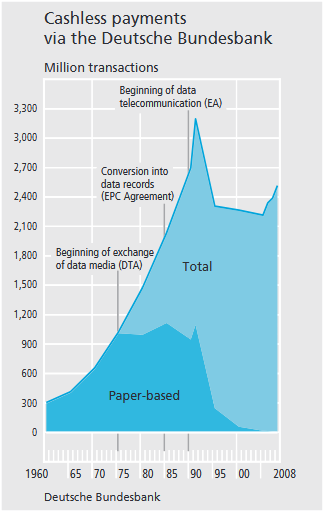
\includegraphics[width=7cm]{Bilder/refrep_DB.png}}
    \caption{Bargeldlose Zahlung über die Deutsche Bundesbank\\ Quelle: Bundesbank, 2009, S.52}
    \label{fig:refrep_DB}
\end{figure}


Laut einer Statistik des \acrfull{ehi} von 2019 bezahlen 48,6\% der deutschen ihre Waren mit Karte, 
wohingegen nur noch 46,9\% der deutschen den klassischen Weg über Bargeld gehen \cite{refart:KSDL} . 
Auch das kontaktlose Bezahlen, bei dem kleine Beträge nicht einmal mit einer \acrfull{pin} bestätigt 
werden müssen, nimmt immer weiter zu. Doch gerade bei dieser Variante ist es sehr einfach im Namen 
eines anderen zu bezahlen, was eine Sicherheitsrisiko darstellt. Diese Tendenz wurde auch von \cite{refart:TDMP} 
in seiner Studie beobachtet, bei der er die meist verbreiteten Zahlungsarten in verschiedenen Regionen
 dieser Welt vergleicht. 


Immer wenn mit Karte bezahlt wird, gehen die Kunden davon aus, dass die Zahlungsabwicklung sicher ist. 
Wie sicher ist das bargeldlose Zahlen heutzutage wirklich? 


\subsection{IT-Schutzziele vom bargeldlosen Zahlungsverfahren}


Vertraulichkeit ist die erste und wichtigste Voraussetzung, das ein solches Zahlungssystem erfüllen muss, 
um neue potenzielle Kunden zu gewinnen. Unter dem Begriff Vertraulichkeit verstehen wir, dass es keine 
unautorisierte Informationsgewinnung gibt \cite{refbook:SWIS}. In dieser Hinsicht sollte ein \acrshort{cba}
so konzipiert werden, dass er einen sicheren Umgang mit den Kundendaten anbietet. Die Interaktion zwischen
einem Kunden und systemkritischen Mechanismen wurde von \cite{refart:HARE} so dargestellt:

\vfill
\begin{figure}[htb]
    \centering{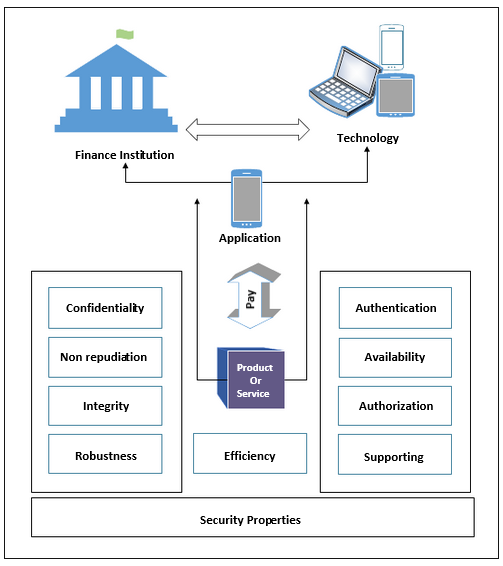
\includegraphics[width=5cm]{Bilder/refark_HARE.png}}
    \caption{Sicherheitseigenschaften von digitalen Zahlungsmethode \\ Quelle: Hassan et al. 2020, S8}
    \label{fig:refark_HARE}
\end{figure}
\vfill

\cite{refart:JTAS} beschreibt didaktisch ein Zahlungsverfahren, dass die Vertraulichkeit gewährleisten kann.
Dieses findet in verschieden 2 getrennte Schritten statt.

Im ersten Schritt sendet der Nutzer seinen Namen. Es wird da einen einen Sitzungsschlüssel generiert und 
eine Anfrage für die Transaktion wird gesendet. Diese Anfrage wird daraufhin an den Händler geschickt, der 
diese wiederrum bearbeitet. Nachdem das abgeschlossen wurde, sendet der Händler seine Antwort an das Zahlungsgerät, 
das wiederrum die Antwort an den Nutzer weiterleitet. 

Im zweiten Schritt wird die Bezahlung Anfrage an das Zahlungsgerät gesendet, die unter anderem den Preis und die 
Uhrzeit enthält. Das Zahlungsgerät leitet die empfangene Nachricht an den Händler weiter. Dieser empfängt die Daten 
und prüft auf Aktualität der Daten. Wenn dieser Test erfolgreich ist, wird wieder eine Nachricht an das Zahlungsgerät 
geschickt. Dieses schickt die Daten dann wiederrum an die Bank, welche überprüft, ob das Geld von dem Konto 
abgebucht werden kann. Wenn das geprüft wurde, wird eine Nachricht an das Zahlungsgerät gesendet, in der steht, 
dass das Geld abgebucht wurde. 

Besonders wichtig ist, dass bei jeder Kommunikation die Daten kryptographisch verschlüsselt werden, sodass es einem 
potenziellen Angreifer nicht möglich ist, Daten zu ändern oder zu entschlüsseln. In den folgenden Abbildungen wird
das oben beschriebene Verfahren dargestellt:

\begin{figure}[H]
    \centering{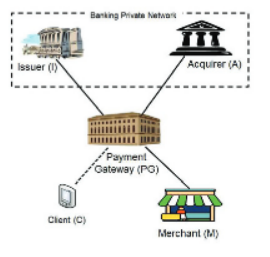
\includegraphics[width=6cm]{Bilder/refart_JTAS_1.png}}
    \caption{Abbildung des Zahlungsverfahren\\ Quelle: Isaac and Zeadally, 2012}
    \label{fig:refart:JTAS}
\end{figure}
%\cite{refart:JTAS}

Das folgende Sequenzdiagramm\footnote{Ein Sequenzdiagramm ist ein Verhaltensdiagramm, welches eine Interaktion
im Sinne der \acrfull{uml} grafisch darstellt \cite{refbook:IASE}.} stellt den 
Nachrichtenaustausch zwischen den Elementen dieser Zahlungsmethode dar:

\vfill
\begin{figure}[H]
    \centering{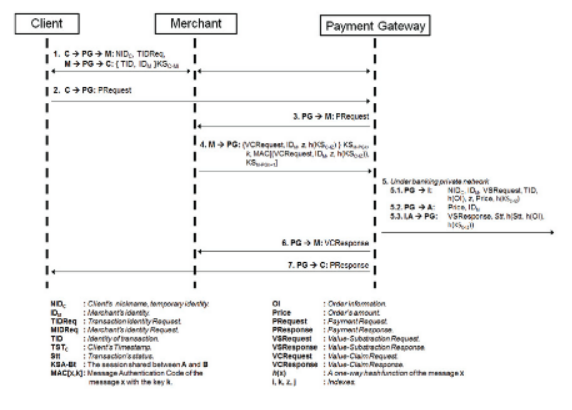
\includegraphics[width=8cm]{Bilder/refart_JTAS_2.png}}
    \caption{Nachrichtenflussaustausch \\ Quelle: Isaac and Zeadally, 2012}
    \label{fig:refart:JTAS_2}
\end{figure}
%\cite{refart:JTAS}

Zudem sollten die weiteren Schutzziele der IT-Sicherheit: Integrität und Authentizität berücksichtigt werden, 
sodass das Zahlungssystem einwandfrei und sicher funktioniert \cite{refip:GMPS}. Eine Zahlungsmethode, bei der 
alle Voraussetzungen erfüllt werden, kann in der Lage sein, das Vertrauen und die Akzeptanz von den Nutzenden 
zu bekommen \cite{refart:HARE}. Besonders im deutschen Markt, spielen die oben genannten Schutzziele eine 
wesentliche Rolle für die Akzeptanz von neuen unbekannten Systemen \cite{refip:DKAM}.

Da wir hier von einem dynamischen und breiten Bereich reden, bei dem es sehr schnell zu Änderungen kommen kann, 
besonders bei den Angriffstechniken, müssen die dazu gehörigen Technologien stets weiterentwickelt und angepasst
werden \cite{refip:NYRS}, um Vertraulichkeitsverlust seitens der Kunden zu vermeiden. Da die Vertraulichkeit noch
nicht zu 100 Prozent gewährleistet werden kann, verweigern viele Kunden das bargeldlose Bezahlen. Aber
wird es jemals eine 100 prozentige Sicherheit geben?

Viele Studien befassen sich mit den verschiedenen Aspekten der Sicherheit bei bargeldlosen Zahlungsmethoden.
Da die Literatur dieses Forschungsfeldes sehr umfangreich ist und da dieses Thema sehr Vielfältig ist 
\cite{refip:GMPS}, sollen hier zwei dieser Technologien in Bezug auf Angriffstechniken und Gegenmaßnahmen 
genauer betrachtet werden: drahtlose Verbindungen mit \acrfull{nfc}\footnote{\acrfull{nfc} ist eine auf Radio Frequenz
basierte Technologie, die der kabelose Austausch von Nachrichten in kürzer Distanz, zwischen vier und zehn cm, 
zwischen elektronischen Gerät, wie Handys, Computer, ermöglicht \cite{refart:NFNK}.} und Smartcards\footnote{Der
Begriff Smartcards bezeichnet eine Plastikkarte mit einem eingebauten Chip, der ein eigenes Betriebssystem, 
einen Mikroprozessor und minimale Funktionalitäten besitzt \cite{refip:JFSB}.}.


